\documentclass{beamer}
\mode<presentation>
\usetheme{CambridgeUS}
\usepackage[russian]{babel}
\usepackage[utf8]{inputenc}
\usepackage[T2A]{fontenc}
\usepackage{sansmathaccent}
\pdfmapfile{+sansmathaccent.map}
\title[Оцифровка]{Аналогово-цифровое и цифроаналоговое преобразование звука}
\author{Наумов Д.А.}
\date[24.02.2014] {Компьютерные музыкальные технологии и звуковой дизайн, 2014}

\begin{document}

%ТИТУЛЬНЫЙ СЛАЙД
\begin{frame}
  \titlepage
\end{frame}
  
%СОДЕРЖАНИЕ ЛЕКЦИИ
\begin{frame}
  \frametitle{Содержание лекции}
  \tableofcontents  
\end{frame}
  
%РАЗДЕЛ 1
\section{АЦП и ЦАП}
\subsection{Аналоговое представление звука}
\begin{frame}

Формы представления звука:
\begin{itemize}
\item в виде непрерывного электрического сигнала;
\item в закодированном цифровом виде. 
\end{itemize}

Аппаратура, в которой рабочим сигналом является непрерывный электрический сигнал, описывающий звуковые колебания, называется {\itshape аналоговой аудиоаппаратурой} (например, бытовой магнитофон, аудиоусилитель, динамик, осциллограф и т.д.), а сам сигнал~--- аналоговым аудиосигналом.

~

Устройство для преобразования звуковых колебаний в электрический (аналоговый) сигнал~--- микрофон, а аналогового сигнала звуковой частоты в звуковые колебания~--- акустический динамик (электродинамический громкоговоритель). 
\end{frame}   

\subsection{Цифровое представление звука}
\begin{frame}
\begin{block}{Цифровой аудиосигнал}
форма (способ) записи аналогового сигнала, т.е. это аналоговый аудиосигнал, представленный некоторым образом в виде дискретных численных значений.
\end{block} 

\begin{block}{Оцифровка}
преобразование аналогового звукового сигнала в цифровой вид. 
\end{block}

\begin{block}{Аналогово-цифровой преобразователь, АЦП}
устройство, предназначенное для осуществления преобразование аналогового звукового сигнала в цифровой вид (Analog-to-Digital Converter~--- АDС). 
\end{block}

Процесс аналогово-цифрового преобразования с помощью АЦП заключается в осуществлении замеров текущих величин амплитуды аналогового сигнала с некоторым временным шагом и последующей записи полученных значений амплитуды в некоторой численной форме.
\end{frame}

\section{Дискретизация и квантование}
\subsection{Дискретизация во времени}
\begin{frame}
\begin{block}{Дискретизация во времени}
процесс регистрации мгновенных значений амплитуды преобразуемого аналогового сигнала (измеряемой в вольтах) через определенные промежутки времени, т.е. с определенным временным шагом, называемым \textit{шагом дискретизации}. 
\end{block}
\centering{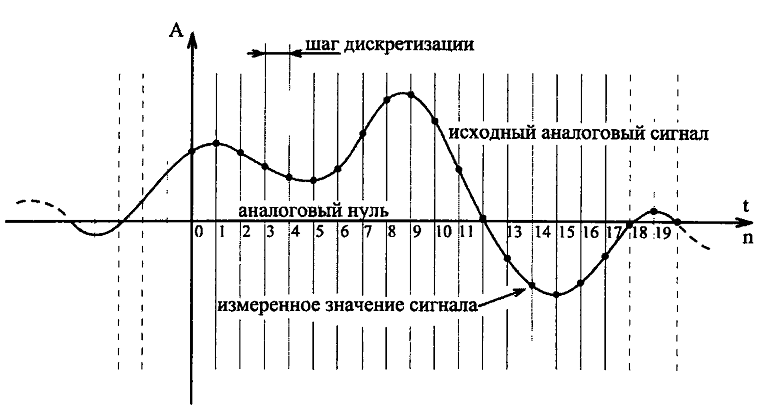
\includegraphics[width=0.9\linewidth]{pic-digital-01}}
\end{frame}

\subsection{Аналоговый нуль}
\begin{frame}
\begin{block}{Частота дискретизации (частота выборки, частота сэмплирования) }
количество осуществляемых в одну секунду замеров амплитуды сигнала, Гц. 
\end{block}

\begin{block}{Аналоговый нуль}
условная линия равновесия ("<тишины">) аналогового сигнала, т.е. линия условного нулевого значения амплитуды
аналогового сигнала, относительно которой совершаются колебания электрического тока, моделирующего колебания звуковой волны (звука).
\end{block}
\begin{itemize}
\item в отсутствии звуковых колебаний на аналоговую цепь подается постоянный потенциал некоторой величины (постоянное напряжение +11 В~--- аналоговый нуль. 
\item звуковые колебания моделируются в аналоговом тракте колебаниями напряжения относительно аналогового нуля.
\end{itemize}
\end{frame}

\subsection{Теорема Котельникова}
\begin{frame}
\begin{block}{Теорема Котельникова}
Согласно этой теореме, аналоговый сигнал с ограниченным спектром может быть точно описан дискретной последовательностью значений его амплитуды, если эти значения следуют с частотой, как минимум вдвое превышающей наивысшую частоту спектра.
\end{block}

\[F_d\geq2F_m\] 

Для того, чтобы оцифрованный сигнал содержал информацию обо всем диапазоне слышимых человеком частот ($0 - 20$ кГц) исходного аналогового сигнала, частота дискретизации при оцифровке должна составлять не менее 40 кГц. Шаг дискретизации = 25 мкс. 

\begin{block}{Проблемы оцифровки}
\begin{itemize}
\item необходимо сохранить точность значений замеров амплитуды сигнала;
\item сделать это нужно в как можно более компактной форме.
\end{itemize} 
\end{block}
\end{frame}

\subsection{Квантование}
\begin{frame}
\begin{itemize}
\item младший квант~--- cамый нижний уровень амплитуды $-1$ у.е.;
\item старший квант~--- cамый верхний уровень амплитуды $+1$ у.е.;
\item кванты пронумеруем от $0$ до $2^N-1$, используя $N$ бит;
\item цифровой нуль расположен ровно между квантами с номерами $2^{N-1}-1$ и $2^{N-1}$.
\end{itemize}
\centering{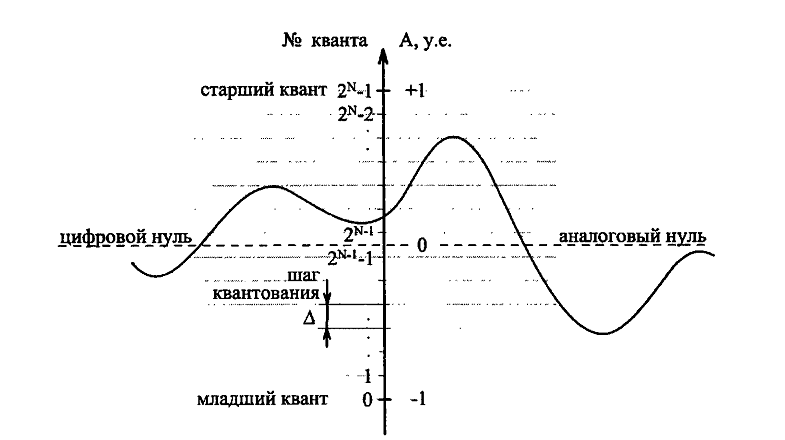
\includegraphics[width=0.75\textwidth]{pic-digital-02}}
\end{frame}

\begin{frame}
В процессе квантования непрерывный аналоговый звуковой сигнал представляется на каждом шаге дискретизации в виде прямоугольных импульсов текущей амплитуды. 
\begin{block}{Квантование исходного аналогового сигнала по амплитуде}
процесс замены реальных (измеренных) значений амплитуды сигнала приближенными значениями с определенной точностью. 
\end{block}
\centering{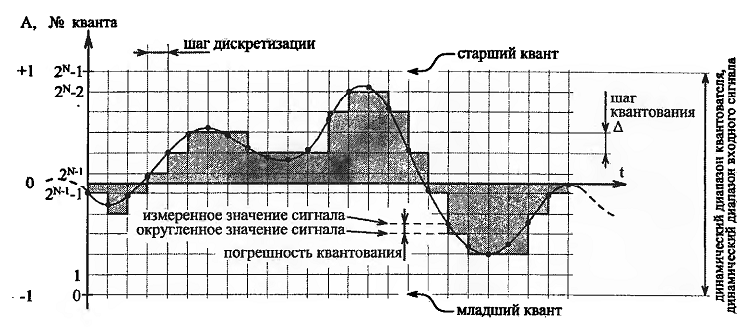
\includegraphics[width=0.75\textwidth]{pic-digital-03}}
\end{frame}

\begin{frame}
Трехбитный квантователь: $N=3$ бит, имеем $2^3=8$ квантов, шаг квантования $\Delta = 2/7$ у.е.
\centering{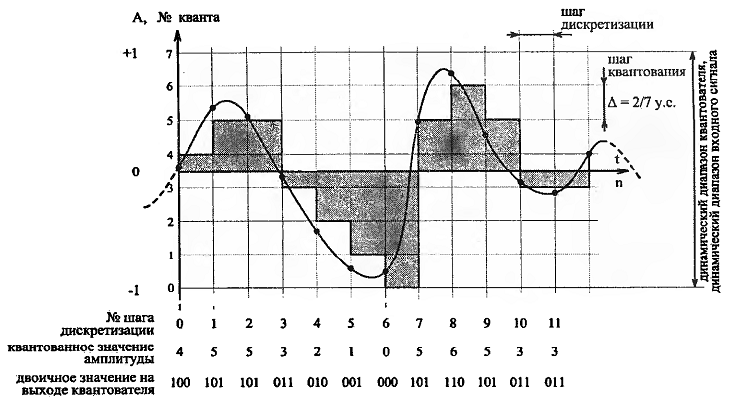
\includegraphics[width=0.75\textwidth]{pic-digital-04}}

Результат квантования: \(4, 5, 5, 3, 2, 1, 0, 5, 6, 5, 3, 3\).

В двоичной форме: \(100, 101, 101, 11, 10, 1, 0, 101, 110, 101, 11, 11\).

На выходе трехбитного квантователя: \(100~101~101~011~010~001~000~101~110~101~011~011\).
\end{frame}

\subsection{Клипирование}
\begin{frame}
\begin{block}{Клипирование (clipping, клиппинг)}
эффект, возникающий тогда, когда динамический диапазон преобразуемого в цифровую форму аналогового сигнала будет превышать динамический диапазон квантователя. 
\end{block}
\centering{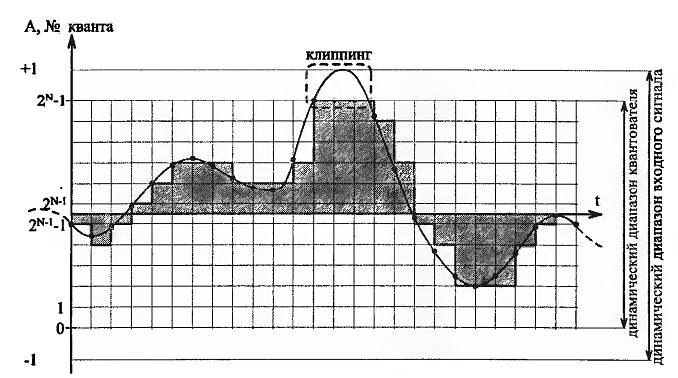
\includegraphics[width=0.75\textwidth]{pic-digital-05}}
\end{frame}

\subsection{DC-offset}
\begin{frame}
Дополнительные проблемы в процессе оцифровки сигнала может вызвать несовпадение уровней аналогового и цифрового нулей, а точнее~--- смещение оси аналогового сигнала относительно цифрового нуля~--- DC-офсет (от англ. "direct current offset"~--- смещение постоянного тока). 
\begin{block}{Сдвиг постоянной составляющей}
расстояние между аналоговым и цифровым нулями. 
\end{block}
\centering{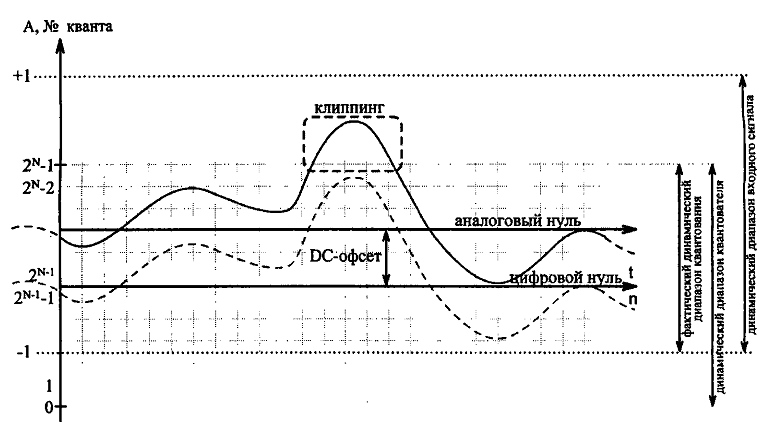
\includegraphics[width=0.75\textwidth]{pic-digital-06}}
\end{frame}

\begin{frame}
СD-DА (Compact Disc Digital Audio)~--- стандарт записи данных на оптических аудио компакт дисках. 

~

Стандарт устанавливает следующие параметры кодирования: двух- или одноканальная запись (т.е. стерео или моно) в формате ИКМ с частотой дискретизации 44,1 кГц и разрядностью квантования 16 бит. 

~

Одна секунда аудио в таком формате занимает 176 400 байт (2 канала $\times$ 44 100 отсчетов в секунду $\times$ 2 байт на отсчет) или 1 411 200 бит. 

~

Говорят, что битрейт (от англ. "<bit rate">~--- "<скорость бита">, "<скорость потока информации">) данных в формате СD-DА составляет 1 411 200 бит/с. 

~

Выходит, что один час аудио в этом формате занимает объем около 600 Мбайт (60 мин $\times$ 60 с $\times$ 2 канала $\times$ 44 100 отсчетов в секунду $\times$ 2 байт на отсчет = 605 Мбайт).
\end{frame}

\section{Цифро-аналоговое преобразование}
\begin{frame}
Процесс цифроаналогового преобразования на практике проходит фактически в два этапа:
\begin{itemize}
\item генерирование ступенчатого аналогового сигнала на основе известной информации об отсчетах цифрового сигнала, взятой, например, из памяти компьютера (ЦАП получает на входе последовательность отсчетов, т.е. цифровых значений сигнала, и выводит на выходе аналоговые импульсы соответствующей величины);
\item сглаживание импульсного аналогового сигнала с помощью аналогового фильтра нижних частот (ФНЧ) с частотой среза, равной половине частоты дискретизации.
\end{itemize}
\centering{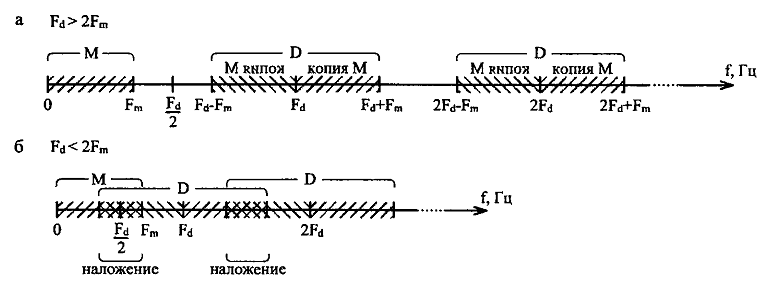
\includegraphics[width=0.75\textwidth]{pic-digital-07}}
\end{frame}

\subsection{Шум квантования}
\begin{frame}
\begin{block}{Шум квантования}
аудиосигнал, составляющий разницу между аналоговым импульсным сигналом, восстановленным из цифрового сигнала на выходе ЦАП, и исходным аналоговым аудиосигналом (до оцифровки).
\end{block}
\centering{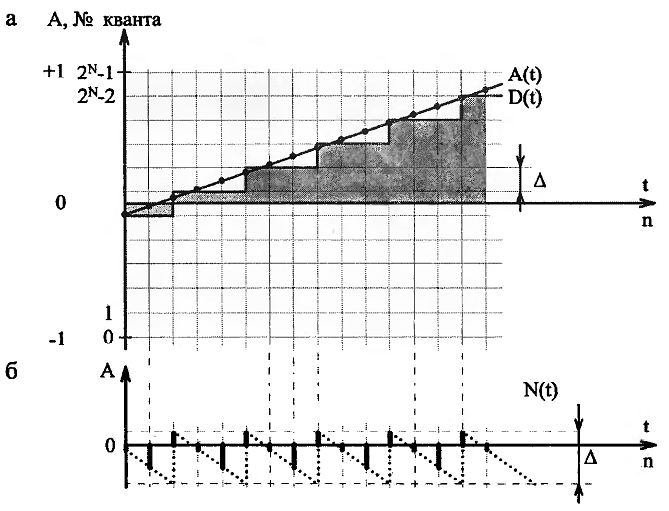
\includegraphics[width=0.7\textwidth]{pic-digital-09}}
\end{frame}
\begin{frame}
Величина шума квантования колеблется в пределах величины $\Delta/2$.

Наибольший уровень шума квантования для данной разрядности квантования $N$:
\[S_i=20 \log(1/k)\text{~дБ,}\]
где $k=2^N$. 
\begin{table}[ht]
  \begin{center}
  \begin{tabular}{|l|c|c|}
  \hline Разрядность, бит & $k$ & Уровень шума квантования, дБ\\
  \hline 1 & 2 & -6 \\  
  \hline 8 & 256 & -48 \\
  \hline 15 & 32 768 & -90 \\
  \hline 16 & 65 536 & -96 \\
  \hline 20 & 1 645 676 & -120 \\ 
  \hline
  \end{tabular}
  \end{center}  
\end{table}
В цифровой аппаратуре 0~дБ (dBFS, Decibel to Full Scale) соответствует максимальному уровню сигнала, а все другие значения откладываются на отрицательной шкале децибелов (при этом положительные значения сигнала в децибелах считаются зашкаливающими).
\end{frame}

\subsection{Дизеринг, гранулярный шум}
\begin{frame}
\begin{block}{Дизеринг}
намеренное "<подмешивание"> к преобразуемому цифровому сигналу слабого по уровню (с амплитудой в пределах до $2\Delta$) псевдослучайного постороннего сигнала, так называемого дизеринг-шума. 
\end{block}
\begin{block}{Формовка шума}(noise shaping) 
преобразование (точнее~--- перераспределение) шума квантования таким образом, чтобы большая часть его энергии расположилась в наименее заметных на слух частотных областях. 
\end{block}
\begin{block}{Джиттер}
осуществление выборки аналогового сигнала в АЦП может происходить не через абсолютно равные промежутки времени, а с некоторыми случайными отклонениями, либо на стадии ЦАП в виде случайных отклонений длительностей (ширины) прямоугольных импульсов от величины шага дискретизации и в отклонениях крутизны фронтов отдельных импульсов.
\end{block}
\end{frame}

\begin{frame}
\begin{block}{Гранулярный шум (granular noise) }
эффект, проявляющийся при имеющей место нестабильности операции округления в процессе квантования сигнала. 
\end{block}
\centering{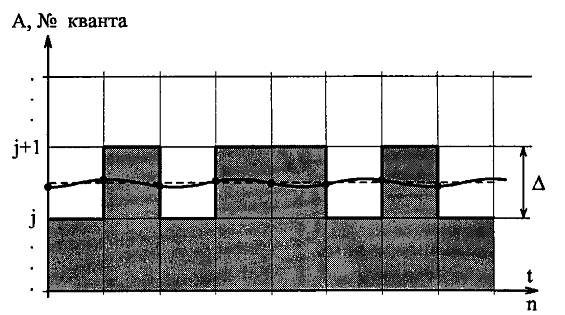
\includegraphics[width=0.75\textwidth]{pic-digital-11}}
\end{frame}

\begin{frame}
Погрешность квантования сигнала в областях со слабой амплитудой оказывается намного более заметной на слух, чем погрешность квантования в областях, где сигнал характеризуется высокими значениями интенсивности.
\begin{block}{Неоднородное квантование}
любой способ квантования, предусматривающий использование непостоянного шага $\Delta (\Delta\neq const)$ с наперед заданным разбиением амплитудной шкалы. 
\end{block}
\centering{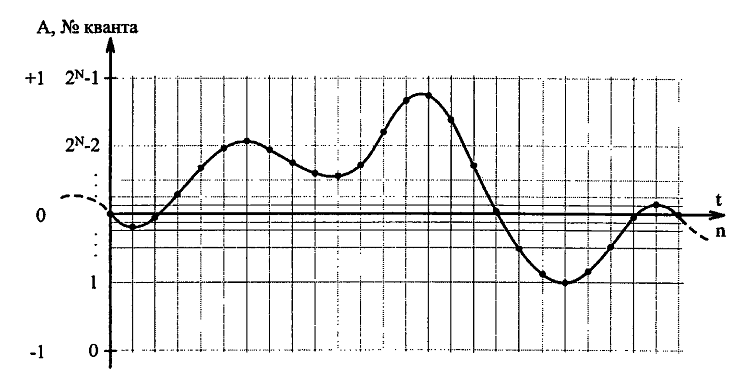
\includegraphics[width=0.75\textwidth]{pic-digital-12}}
\end{frame}

\section[Аналоговое VS Цифровое]{Сравнение аналоговой и цифровой форм представления звука}
Три различные трактовки понятия "<качества звука">:
\begin{enumerate}
\item какая форма представления звуковых колебаний обеспечивает сравнительно более точное приближение к звучанию источника звука;
  \begin{itemize}
     \item чем меньше тракт, тем лучше;
     \item гармонические и негармонические искажения.
  \end{itemize}
\item какая форма представления звуковых колебаний обеспечивает наиболее приятное звучание с точки зрения слушателя;
  \begin{itemize}
     \item Hi-Fi и Hi-End;
     \item кодирование с потерями.
  \end{itemize}
\item какая форма представления звуковых колебаний обеспечивает максимальную компактность, сохранность и предоставляет эффективную возможность преобразования аудиоданных (их монтажа, коррекции и пр.).
  \begin{itemize}
     \item ограниченность носителей аналоговой информации;
     \item неограниченный возможности преобразования цифровой информации.
  \end{itemize}
\end{enumerate}


\end{document}
